\documentclass{school}
% using the school template from https://github.com/re1/latex-templates
\title{Stochastik}
\subject{Angewandte Mathematik}
\author{Markus Reichl}

\begin{document}
\thispagestyle{fancy}

\newacronym{hgv}{HgV}{Hypergeometrische Verteilung}
\newacronym{bv}{BV}{Binomialverteilung}
\newacronym{nv}{NV}{Normalverteilung}
\newacronym{snv}{SNV}{Standardisierte Normalverteilung}
\newacronym{zsb}{ZSB}{Zufallsstreubereich}

\newpage
\section{Statistik}
\subsection{Begriffe}
\begin{tabularx}{\textwidth}{X c l}
Mittelwert & $\bar{x} = \frac{Summe}{Anzahl}$ & \small{Durchschnittlicher Wert einer Liste.}\\
&& \footnotesize{$\to$ maxima: \verb|mean(<<liste>>)|}\\
Standardabweichung & $\sigma = \sqrt{\frac{1}{n} \sum_{i=1}^{n} (x_i - \bar{x})^2}$ & \small{Mittlere Abweichung vom Mittelwert.}\\
&& \footnotesize{$\to$ maxima: \verb|std(<<liste>>)|}\\
Varianz & $\sigma^2$ & \small{Mittlere quadratische Abweichung vom Mittelwert.}\\
&& \footnotesize{$\to$ maxima: \verb|var(<<liste>>)|}\\
Median & $\hat{x}$ & \small{Mittlerer Wert einer geordneten Liste.}\\
&& \footnotesize{$\to$ maxima: \verb|median(<<liste>>|}\\
Minimum & $x_0$ & \small{Erster Wert einer geordneten Liste.}\\
&& \footnotesize{$\to$ maxima: \verb|min(<<liste>>)|}\\
Maximum & $x_n$ & \small{Letzter Wert einer geordneten Liste.}\\
&& \footnotesize{$\to$ maxima: \verb|max(<<liste>>)|}\\
Spannweite & $r = x_0 - x_n$ & \small{Differenz zwischen Minimum und Maximum.}\\
&& \footnotesize{$\to$ maxima: \verb|range(<<liste>>|}\\
1. Quartil & $q_1$ & \small{Median der Werte vor dem Median einer geordneten Liste.}\\
&& \footnotesize{$\to$ maxima: \verb|quantile(<<liste>>, 0.25)|}\\
2. Quartil & $q_2 = \hat{x}$ & \small{Median einer geordneten Liste.}\\
&& \footnotesize{$\to$ maxima: \verb|quantile(<<liste>>, 0.5)|}\\
3. Quartil & $q_3$ & \small{Median der Werte nach dem Median einer geordneten Liste.}\\
&& \footnotesize{$\to$ maxima: \verb|quantile(<<liste>>, 0.75|}
\end{tabularx}

\subsubsection{Boxplot}
Aus dem Boxplot lassen sich die Quartile, der Median, sowie Minimum und Maximum auslesen. Dabei wird eine Skala vom Minimum zum Maximum gezogen und eine Box vom 1. bis zum 3. Quartil gespannt, die vom Median geteilt wird. Zusätzlich können auch Ausreißer vor oder nach dem Boxplot gezeichnet werden.
\begin{figure}[h]
	\centering
	\includegraphics[width=0.5\textwidth]{boxplot.png}
	\caption{Boxplot}
\end{figure}

{\footnotesize $\to$ maxima: \verb|boxplot(<<liste>>, box_orientation=horizontal)|}

\newpage
\section{Wahrscheinlichkeit}
Der Zufall unterliegt Regeln, die erst bei einer großen Anzahl von Versuchen sichtbar werden.
Ein Zufallsexperiment muss $n$ Mal durchgeführt werden, um zu erkennen, dass das Ereignis $A$ $k$ Mal auftritt.

Nach einer ausreichenden Zahl von Versuchen kann man als Schätzwert für die Wahrscheinlichkeit $P(A)$, die Anzahl der Ereignisse $k$ relativ zur Anzahl der Versuche $n$ nehmen.
$$P(A) = \frac{k}{n}$$
{\footnotesize $$0 \leqslant P(A) \leqslant 1$$}
\begin{vardefs}
\addvardef{$P(A)$}{Wahrscheinlichkeit}
\addvardef{$A$}{Ereignis}
\addvardef{$k$}{Anzahl der Ereignisse}
\addvardef{$n$}{Anzahl der Versuche}
\end{vardefs}

\subsection{Laplace Experiment}
Gilt für ein Zufallsexperiment, dass
\begin{outline}
\1 endlich viele Ereignisse existieren und
\1 jedes Ereignis gleich wahrscheinlich ist,
\end{outline}
kann man ein Laplace Experiment durchführen. Man unterscheidet dabei die Zahl der günstigen $g$ und der möglichen $m$ Fälle für ein Ereignis $A$. Die Wahrscheinlichkeit $P(A)$ für ein Ereignis $A$ ist als Quotient der günstigen $g$ und der möglichen $m$ Fälle definiert.
$$P(A) = \frac{g}{m}$$

\subsection{Zusammengesetzte Ereignisse}
2 Ereignisse $A, B$ sollen zu einem Ereignis $C$ zusammengesetzt werden.
\begin{center}
\begin{tabularx}{0.5\textwidth}{c c c}
	$A$ UND $B$ & bzw. & $A$ ODER $B$\\
	{\small ($A$ und $B$ zugleich)} & & {\small (mindestens $A$ oder $B$)}
\end{tabularx}
\end{center}

\begin{outline}
\1 \textbf{Gegenwahrscheinlichkeit}
$$P(\bar{A}) = 1 - P(A) \quad \bar{A} \quad \dots \quad \text{„Non-A“}$$

\1 \textbf{Unvereinbarkeit}
$$P(A_{\text{UND}}B) = 0$$

\1 \textbf{Additionssatz {\footnotesize(ODER-Regel)}}
$$P(A_{\text{ODER}}B) = P(A) + P(B) - P(A_{\text{UND}}B) \quad \text{wenn A und B beliebig}$$
$$P(A_{\text{ODER}}B) = P(A) + P(B) \quad \text{wenn A und B unvereinbar}$$

\1 \textbf{Multiplikationssatz \small{(UND-Regel)}}
$$P(A_{\text{UND}}B) = P(A) * P(B_{\text{ODER}}A) \quad \text{wenn A und B beliebig}$$
$$P(A_{\text{UND}}B) = P(A) * P(B) \quad \text{wenn A und B unvereinbar}$$
\end{outline}

\newpage
\subsection{Bernoulli Versuch \normalsize{(Pfade)}}
\paragraph{1. Pfadregel \small{(UND-Regel)}} Die Wahrscheinlichkeit eines Ereignisses ist gleich dem Produkt der Wahrscheinlichkeiten entlang seines Pfades.
\paragraph{2. Pfadregel \small{(ODER-Regel)}} Die Wahrscheinlichkeit eines Ereignisses ist gleich der Summe der Wahrscheinlichkeiten seiner Pfade.

\subsubsection{Baumdiagramm}
Der Bernoulli Versuch kann über sogenannte Baumdiagramme dargestellt werden. In diesem Beispiel werden zwei Münzen geworfen und es soll die Wahrscheinlichkeit berechnet werden, zu der mindestens einmal Zahl fällt.

\begin{figure}[h]
	\centering
	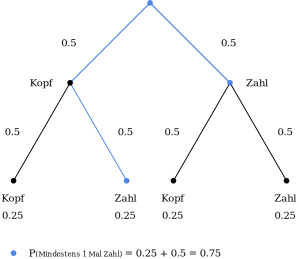
\includegraphics[width=0.5\textwidth]{tree.png}
	\caption{Baumdiagramm}
\end{figure}

Die Wahrscheinlichkeit bei einem Wurf Zahl zu werfen, liegt bei 50\%. Am linken Pfad wird erst ein Kopf und dann eine Zahl, am rechten Pfad gleich eine Zahl geworfen. Zur Berechnung der Wahrscheinlichkeit werden nun die Produkte der Pfade aufsummiert.

$$P_{\text{(Mindestens 1 Mal Zahl)}} = \text{Kopf} * \text{Zahl} + \text{Zahl} = 0.5 * 0.5 + 0.5 = 0.75$$
\begin{center}
$\to$ Zu 75\% wird mindestens einmal Zahl geworfen.
\end{center}

\newpage
\subsection{Abzähltechniken}
\subsubsection{Permutation}
Es seien 4 Personen gegeben und es wird die Anzahl verschiedener Reihenfolgen gesucht. Jede Person kann nur an einer Position stehen, es handelt sich also um ein \textit{ziehen ohne zurücklegen}.
\\\\
Nach jeder Auswahl einer Position stehen eine Person und ein Platz weniger zur Verfügung.

{\small \begin{tabular}{l l l l l}
1. & 2. & 3. & 4. & Position\\
4 & 3 & 2 & 1 & Möglichkeiten
\end{tabular}}
\\\\
Es bestehen also $4 * 3 * 2 * 1$ Möglichkeiten (Permutationen) oder $4$ Fakultät ($4!$).\\
Die Anzahl der Permutationen von $n$ Elementen entspricht also $n! = \sum_{i=0}^{n - 1} n-i$.
\\\\
In Maxima kann die Fakultät mittels \verb|factorial(n)| berechnet werden.

\subsubsection{Kombination}
Aus $n=7$ Personen sollen $k=3$ Personen ausgewählt werden. Die Reihenfolge ist dabei belanglos, es handelt sich also um ein \textit{ziehen mit zurücklegen}.

{\small \begin{tabular}{l l}
$7 * 6 * 5$ & sind wählbar\\
$3 * 2 * 1$ & sind gleich für jede Auswahl
\end{tabular}}
\\\\
Es bestehen also $\frac{7 * 6 * 5}{3 * 2 * 1} = \frac{210}{6} = 35$ Möglichkeiten.
Allgemein ist die Kombination als $\frac{n * (n-1) \text{\dots} (n - k + 1)}{1 \text{\dots} k}$ definiert, was dem Binomialkoeffizienten entspricht.

\paragraph{Binomialkoeffizient}
$$\binom{n}{k} = \frac{n!}{(n-k)! * k!}$$

In Maxima kann der Binomialkoeffizient mittels \verb|binomial(n, k)| berechnet werden.

\subsubsection{Variation \normalsize{(Geordnete Auswahl)}}
Aus $n=7$ Personen sollen $k=3$ ausgewählt werden. Die Reihenfolge der Kombination ist dabei zu beachten, es handelt sich also um ein \textit{ziehen ohne zurücklegen}.

{\small \begin{tabular}{l l l l}
1. & 2. & 3. & Position\\
$7$ & $6$ & $5$ & $\rightarrow 7 * 6 * 5$ Möglichkeiten
\end{tabular}}
\\\\
Die Variation kann auch anhand der Kombination berechnet werden.
$$\binom{7}{3} * 3! = 7 * 6 * 5 = 210 \text{~Variationen}$$

\newpage
\section{Verteilung}
\subsection{Funktionen}
\paragraph{Verteilungsfunktion $G(x)$}
Die Zufallsvariable nimmt einen Wert kleiner gleich $x$ an.
$$P(\leqslant x) = G(x)$$
$$P(\geqslant x) = 1 - G(x - 1)$$

\paragraph{Wahrscheinlichkeitsfunktion $g(x)$}
Die Zufallsvariable nimmt den Wert $x$ an.
$$P(x) = g(x) = G(x) - G(x - 1)$$

\subsection{Diskrete Verteilung}
Eine Wahrscheinlichkeitsverteilung ist diskret, wenn die Menge entweder
\begin{outline}
\1 endlich
\1 unendlich aber abzählbar oder
\1 beliebig definiert ist und eine abzählbare Zahl von positiven Elementen aufweist ($P(M) = 1$).
\end{outline}
Die Menge besteht dabei meist aus natürlichen Zahlen $\mathbb{N}$.

\subsubsection{\gls{hgv}}
Eine Grundgesamtheit $N$ enthält $K$ Merkmalsträger\footnote{Im Qualitätsmanagement werden Merkmalsträger auch als Defekte $D$ und die Grundmenge als Prüflos bezeichnet. Im deutschen Sprachraum ist für die Merkmalsträger die Variable $M$ gängig.}, die zu einer Wahrscheinlichkeit $P$, $k$ Mal in einer Stichprobe $n$ zu finden sind.
Durch das Ziehen der Stichprobe wird die Grundgesamtheit verändert, es handelt sich also um ein \textbf{Ziehen ohne Zurücklegen}.

$$P(k) = \frac{\binom{K}{k}\binom{N-K}{n-k}}{\binom{N}{n}}$$
{\footnotesize $$x \leqslant K \quad n-k \leqslant N-K\footnote{Gilt $k \leqslant K \quad n-k \leqslant N-K$ nicht, ist $P(k) = 0$}$$}
\begin{vardefs}
\addvardef{$P(k)$}{Wahrscheinlichkeit, dass $k$ Ereignisse auftreten}
\addvardef{$N$}{Grundmenge}
\addvardef{$K$}{Merkmalsträger}
\addvardef{$k$}{Anzahl der Ereignisse}
\addvardef{$n$}{Umfang der Stichprobe}
\end{vardefs}~\\
Für die \gls{hgv} kann ein Erwartungswert $\mu$ gefunden werden.
$$\mu = n * \frac{K}{N}$$

\newpage
\subsubsection{\gls{bv}}
In einer Stichprobe $n$ sind zu einer Wahrscheinlichkeit $P$, $k$ Merkmalsträger zu finden. Diese treten immer zur Wahrscheinlichkeit $p$\footnote{$p$ wird meist einzeln angegeben, kann jedoch auch als Quotient der Merkmalsträger $K$ und der Grundmenge $N$ berechnet werden. $$p = \frac{K}{N}$$} auf, es handelt sich also um ein \textbf{Ziehen mit Zurücklegen}.

$$P(k) = \binom{n}{k} * p^k * (1 - p)^{n-k}$$
\begin{vardefs}
\addvardef{$P(k)$}{Wahrscheinlichkeit, dass $k$ Ereignisse auftreten}
\addvardef{$k$}{Anzahl der Ereignisse}
\addvardef{$n$}{Umfang der Stichprobe}
\addvardef{$p$}{Wahrscheinlichkeit eines Ereignisses}
\end{vardefs}~\\
Für die \gls{bv} kann ein Erwartungswert $\mu$ gefunden werden.
$$\mu = n * p$$

\subsection{Stetige Verteilung}
Im Gegensatz zur diskreten Verteilung kann die Menge beliebige Werte, innerhalb eines definierten Intervalls annehmen. Die Verteilungsfunktion von $P$ ist dabei stetig, mit $P \in \mathbb{R}$.

\subsubsection{\gls{nv}}
Eine stetige Zufallsvariable $x$ mit der Wahrscheinlichkeitsdichte $g : \mathbb{R} \to \mathbb{R}_{\>0}$, definiert als
$$g(x) = \frac{1}{\sigma\sqrt{2\pi}} * e^{-\frac{(x-\mu)^2}{2\sigma}}$$
\begin{vardefs}
\addvardef{$g(x)$}{Wahrscheinlichkeitsdichte}
\addvardef{$x$}{Zufallsvariable}
\addvardef{$\mu$}{Erwartungswert}
\addvardef{$\sigma$}{Standardabweichung}
\end{vardefs}
heißt normalverteilt. Die resultierende Kurve wird als „Gaußsche Glockenkurve“ bezeichnet und nimmt im Integral $\int_{-\infty}^{+\infty}$ immer den Wert $1$ an.

\newpage
\paragraph{Eigenschaften}
\begin{outline}
\1 Symmetrisch zu $\mu$
\1 Keine Nullstellen
\1 2 Wendepunkte \quad $\mu \pm \sigma$
\1 Eine Veränderung von $\mu$ verschiebt die Kurve an der x-Achse
\1 Eine Veränderung von $\sigma$ verbreitert die Kurve
\1 Die Fläche unter der Kurve ist immer $1$
\1 Die Wahrscheinlichkeit, dass ein Merkmal $\leqslant x_0$ ist, entspricht der Fläche unter der Kurve zwischen $-\infty$ bis $x_0$
$$\int_{-\infty}^{x_0}g(x;\mu,\sigma)dx$$
\1 Die Wahrscheinlichkeit, dass ein Merkmal zwischen $a$ und $b$ ist, entspricht der Fläche unter der Kurve zwischen $a$ bis $b$
$$\int_{a}^{b}g(x;\mu,\sigma)dx$$
\1 Die Dichtefunktion ist nicht analytisch, sondern nur numerisch zu berechnen
\end{outline}

\subsubsection{\gls{snv}}~\\
Eine \gls{nv} ist standardisiert wenn der Erwartungswert $\mu = 0$ und die Standardabweichung $\sigma = 1$ ist. Durch eine z-Transformation kann aus jeder beliebigen \gls{nv} eine \gls{snv}gebildet werden.
$$g(x;0,1) = \varphi(z)$$
$$z = \frac{x-\mu}{\sigma}$$

\newpage
\section{Beurteilende Statistik}
Mithilfe der beurteilenden Statistik wird aus empirisch gewonnenen Daten auf unbekannte Größen, wie Wahrscheinlichkeiten und Erwartungswerte geschlossen.

Speziell geht es dabei um den Zusammenhang zwischen Grundgesamtheit und Stichprobe.

\subsection{\gls{zsb}}
Der \gls{zsb} gibt an, zu welcher Wahrscheinlichkeit eine Stichprobe in einem bestimmten Bereich liegt. Diese Wahrscheinlichkeit ist abhängig
\begin{outline}
\1 von den Eigenschaften der Grundgesamtheit
	\2 z.B.: $\mu$, $\sigma$
\1 vom Zufall
\end{outline}

\paragraph{\gls{zsb} von $\mu,\sigma$}
\begin{outline}
\1 Zweiseitig begrenzter \gls{zsb}
$$x_{o,u} = \mu \pm z_{1 - \frac{\alpha}{2}} * \sigma$$
\1 Einseitig begrenzter \gls{zsb}
$$x_{o} = \mu + z_{1 - \alpha} * \sigma$$
$$x_{u} = \mu - z_{1 - \alpha} * \sigma$$
\end{outline}

\paragraph{\gls{zsb} für Stichprobenmittelwerte}
\begin{outline}
\1 Zweiseitig begrenzter \gls{zsb}
$$\bar{x_{o,u}} = \mu \pm z_{1 - \frac{\alpha}{2}} * \frac{\sigma}{\sqrt{n}}$$
\1 Einseitig begrenzter \gls{zsb}
$$\bar{x_{o}} = \mu + z_{1 - \alpha} * \frac{\sigma}{\sqrt{n}}$$
$$\bar{x_{u}} = \mu - z_{1 - \alpha} * \frac{\sigma}{\sqrt{n}}$$
\end{outline}

\begin{vardefs}
\addvardef{$x$}{\acrfull{zsb}}
\addvardef{$\bar{x}$}{Mittelwert}
\addvardef{$o$}{nach oben}
\addvardef{$u$}{nach unten}
\addvardef{$z$}{Zufallsvariable der Standardnormalverteilung}
\addvardef{$\alpha$}{Irrtumswahrscheinlichkeit (Signifikanzniveau)}
\addvardef{$\mu$}{Erwartungswert aus Grundgesamtheit}
\addvardef{$\sigma$}{Standardabweichung aus Grundgesamtheit}
\addvardef{$n$}{Umfang der Stichprobe}
\end{vardefs}

\newpage
\subsection{Vertrauensbereich (Konfidenzintervall)}
Der Vertrauensbereich gibt die Wahrscheinlichkeit an, zu der ein Parameter der Grundgesamtheit in einem bestimmten Bereich liegt.

\paragraph{Vertrauensbereich für $\mu$}
\begin{outline}
\1 $\sigma$ bekannt
$$\mu_{o,u} = \bar{x} \pm z_{1-\frac{\alpha}{2}} * \frac{\sigma}{\sqrt{n}}$$
\1 $\sigma$ unbekannt
$$\mu_{o,u} = \bar{x} \pm t_{f;1-\frac{\alpha}{2}} * \frac{s}{\sqrt{n}}$$
\end{outline}
\paragraph{Vertrauensbereich für $\sigma$}
$$\sigma_o = s * \sqrt{\frac{f}{x^2_{f;\frac{\alpha}{2}}}}\quad;\quad\sigma_u = s * \sqrt{\frac{f}{x^2_{f;1-\frac{\alpha}{2}}}}$$

\begin{vardefs}
\addvardef{$\bar{x}$}{Mittelwert}
\addvardef{$o$}{nach oben}
\addvardef{$u$}{nach unten}
\addvardef{$z$}{Zufallsvariable der Standardnormalverteilung}
\addvardef{$t$}{Zufallsvariable der Student-Verteilung}
\addvardef{$f$}{Freiheitsgrad $f = n - 1$}
\addvardef{$\alpha$}{Irrtumswahrscheinlichkeit (Signifikanzniveau)}
\addvardef{$\mu$}{Erwartungswert aus Grundgesamtheit}
\addvardef{$\sigma$}{Standardabweichung aus Grundgesamtheit}
\addvardef{$n$}{Umfang der Stichprobe}
\end{vardefs}



% Basic Figure
% \begin{figure}[h]
%	 \centering
% 	 \includegraphics[height=4cm]{image.jpg}
% 	 \caption{Caption}
% \end{figure}

% Basic bibiography
% \begin{thebibliography}{9}
% \bibitem{faz} faz.net, Vergewaltigung live auf Facebook gezeigt \\ http://www.faz.net/aktuell/gesellschaft/kriminalitaet/vergewaltigung-live-auf-facebook-gezeigt-14936872.html
% \end{thebibliography}

% List of figures
% \listoffigures
\end{document}